%%%%%%%%%%%%%%%%%%%%%%%%%%%%%%%%%%%%%%%%%%%%%%%%%%%%%%%%%%%%%%%%%%%%%%%
% BAB 3
%%%%%%%%%%%%%%%%%%%%%%%%%%%%%%%%%%%%%%%%%%%%%%%%%%%%%%%%%%%%%%%%%%%%%%%

\mychapter{3}{BAB 3 METODOLOGI}

Pada bab ini akan dijelaskan langkah-langkah
penelitian. Langkah pertama diawali dengan studi literatur. Langkah selanjutnya
diikuti dengan rekayasa kebutuhan, perancangan, implementasi dan pengujian yang
merupakan urutan tahapan pada pengembangan sistem yang menggunakan model
\emph{waterfall}. Pemilihan model \emph{waterfall} dalam pengembangan sistem
pada penelitian ini disebabkan kebutuhan sistem yang sudah dapat didefinisikan
dengan baik pada tahap awal pengembangan sistem. Pengujian merupakan langkah
terakhir dalam pengembangan sistem pada penelitian ini, hal ini sesuai dengan
rumusan masalah penelitian. Langkah terakhir penelitian
ditutup dengan penarikan kesimpulan dan saran. Langkah-langkah tersebut dapat
dilihat pada pada Gambar~\ref{fig:diagram-alir}.

\begin{figure}[tph]
  \centering
  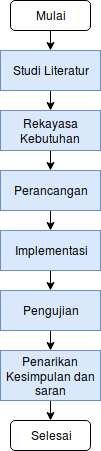
\includegraphics[width=.17\linewidth]{img/diagram-metodologi}
  \caption{Diagram alir metodologi}\label{fig:diagram-alir}
\end{figure}

\section{Studi Literatur}

Studi literatur dibutuhkan untuk mendalami teori-teori dan urgensi
tentang plagiarisme lebih dalam. Selain itu, studi literatur juga
dibutuhkan untuk mendalami teori rekayasa perangkat lunak untuk
mengembangkan perangkat lunak pencegah plagiarisme dengan menggunakan
metode \emph{snapshotting} dan \emph{user activity logging}. Sumber
dari literatur tersebut berasal dari jurnal, buku, situs resmi dan
dokumentasi perangkat lunak yang digunakan. Daftar literatur yang
dipelajari terkait dengan:

\begin{enumerate}
\item Penelitian-penelitian sebelumnya yang terkait dengan plagiarisme
\item Metode \emph{user activity logging, snapshotting} dan \emph{edit-distance algorithm}
\item Teori pengembangan perangkat lunak, yang di dalamnya meliputi
  teori rekayasa kebutuhan, perancangan, implementasi, dan pengujian
\item Teknologi yang digunakan dalam penelitian
\end{enumerate}

\section{Rekayasa Kebutuhan}

Rekayasa kebutuhan merupakan kumpulan tugas dan teknik untuk memahami
kebutuhan. Terdapat empat tahapan dalam rekayasa kebutuhan, yaitu
analisis kebutuhan, spesifikasi kebutuhan, manajemen kebutuhan, dan
pemodelan kebutuhan. Penjelasan tentang tahapan-tahapan yang dilakukan
dalam rekayasa kebutuhan adalah sebagai berikut:

\begin{enumerate}[
leftmargin=0pt, itemindent=20pt,
labelwidth=15pt, labelsep=5pt, listparindent=0.7cm,
align=left]

\item Analisis kebutuhan

  % - metode ihantola: waktu mulai + selesai, alamat IP
  % - kekurangan ihantola (``future work''') <- diperkuat oleh penelitian Leung: bantuan external
  % - sistem TMC Hellas yang platform dependend
  Pada tahapan ini dilakukan penggalian kebutuhan sistem. Kebutuhan fungsional
  sistem didapatkan dari:

  \begin{enumerate}
  \item Metode yang telah digunakan pada penelitian
    \parencite{hellas2017plagiarism}.
  \item ``\emph{Future work}'' penelitian \textcite{hellas2017plagiarism}, dan
    penelitian \textcite{leung2017instructional} yang memaparkan cara-cara
    plagiarisme di mana cara-cara tersebut belum dapat ditangani oleh penelitian
    \textcite{hellas2017plagiarism}.
  \item Kelemahan dari penelitian \textcite{hellas2017plagiarism} yang akan disempurnakan.
  \end{enumerate}

  Pada sumber kebutuhan fungsional pertama didapatkan kebutuhan fungsional untuk
  merekam waktu mulai pengerjaan, waktu selesai pengerjaan, rekaman alamat
  \emph{IP}, dan menghitung nilai \emph{edit-distance} pada berkas tugas.  Sumber
  kebutuhan fungsional kedua dan ketiga menghasilkan kebutuhan fungsional untuk
  merekam perubahan berkas tugas dengan metode \emph{snapshotting}, merekam
  aktivitas siswa menggunakan metode \emph{user activity logging}, dan
  mengembangkan sistem dengan sifat \emph{agnostic} agar tidak terikat pada
  \emph{platform} tertentu. Komponen aktivitas siswa yang direkam adalah seluruh
  \emph{window}, \emph{window} yang sedang aktif, nama \emph{login}, dan nama
  \emph{device}.

  Kebutuhan non-fungsional didapatkan dari batasan sistem yang hanya dapat
  berjalan pada sistem operasi \emph{GNU/Linux}, terdapat berbagai macam
  \emph{desktop environment} pada sistem operasi \emph{GNU/Linux} sehingga
  sistem yang dibangun harus \emph{compatible} dengan enam \emph{desktop
    environment} yang umum digunakan. Keenam \emph{desktop environment} tersebut
  adalah \emph{GNOME, KDE, XFCE, Unity, Cinnamon} dan \emph{Phanteon}.

\item Spesifikasi kebutuhan

  Pada tahapan ini hasil dari analisis kebutuhan pada tahapan
  sebelumnya dijelaskan secara lebih mendetail dengan jelas, tidak
  ambigu, mudah dipahami, dan konsisten. Kebutuhan fungsional
  mendeskripsikan apa yang dapat dilakukan oleh sistem yang dibangun
  dan kebutuhan non-fungsional mendeskripsikan batasan atau
  kualitas dari sistem yang dibangun.

\item Manajemen kebutuhan

  Tahapan ini dilakukan untuk memudahkan dalam mengidentifikasi, mengontrol
  dan melacak kebutuhan. Maka pada tahapan ini dilakukan
  kodefikasi pada kebutuhan-kebutuhan yang ada. Kode LUP-F-1 dan
  LUPR-F-1 untuk kebutuhan fungsional, LUPR-NF-1 dan LUPR-NR-1 untuk
  kebutuhan non-fungsional.

\item Pemodelan kebutuhan

  Tahap terakhir adalah pemodelan kebutuhan. Untuk menggambarkan fungsionalitas
  dan batasan sistem secara visual, penelitian ini menggunakan alat bantu
  \emph{use case diagram}, sedangkan untuk menjelaskan skenario interaksi antar aktor
  dan sistem secara mendetail, penelitian ini menggunakan alat bantu \emph{use
    case scenario}. Penggunaan kedua diagram tersebut dalam tahapan ini dapat
  memodelkan kebutuhan sistem baik secara visual (\emph{use case diagram})
  maupun secara tekstual dengan detail (\emph{use case scenario}).

\end{enumerate}

\section{Perancangan}

Tahapan perancangan sistem menjelaskan tentang rancangan sistem yang
akan dibangun berdasarkan hasil rekayasa kebutuhan pada tahapan
sebelumnya. Rancangan ini nantinya akan menjadi acuan pada tahap
implementasi dan pengujian. Tahap-tahap yang dilakukan pada perancangan
sistem adalah:

\begin{enumerate}[
leftmargin=0pt, itemindent=20pt,
labelwidth=15pt, labelsep=5pt, listparindent=0.7cm,
align=left]

\item Perancangan arsitektur

  Sistem akan dibangun dengan arsitektur \emph{Model-View-Controller}
  (\emph{MVC}). Arsitektur \emph{MVC} dipilih agar komponen fungsionalitas
  sistem terpisah dari komponen antarmuka sistem. Hal ini memudahkan
  pengembangan selanjutnya, karena pengembang
  cukup fokus pada masing-masing komponen yang terpisah. Arsitektur ini juga
  memudahkan proses \emph{porting} maupun penggantian antarmuka, karena
  pengembang cukup fokus pada komponen antarmuka sistem. Untuk menggambarkan
  interaksi yang terjadi antar komponen pada sistem, penelitian ini menggunakan
  alat bantu \emph{sequence digaram}. Terdapat tiga sampel \emph{sequence
    diagram} yang akan dipaparkan pada tahapan ini. Untuk menggambarkan struktur
  sistem dan relasi antar komponen pada sistem, penelitian ini menggunakan alat
  bantu \emph{class diagram}.

\item Perancangan komponen

  Pada tahapan ini komponen sistem akan dirancang menggunakan
  \emph{pseudocode}. \emph{Pseudocode} inilah yang nantinya menjadi
  acuan pada tahapan implementasi. Pada tahapan ini terdapat tiga
  sampel perancangan komponen yang akan dipaparkan.

\item Perancangan antarmuka

  Pada tahapan ini rancangan antarmuka sistem dan tata letak komponen antarmuka
  di dalamnya digambarkan dengan gambaran sederhana. Perancangan antarmuka
  dilakukan dengan kakas bantu \emph{draw.io}. Terdapat tiga
  sampel perancangan antarmuka yang akan dipaparkan pada tahapan ini.

\end{enumerate}

\section{Implementasi}

Pada tahapan implementasi, hasil perancangan pada tahapan sebelumnya
diimplementasikan, terdapat dua tahapan dalam implementasi yaitu:

\begin{enumerate}[
leftmargin=0pt, itemindent=20pt,
labelwidth=15pt, labelsep=5pt, listparindent=0.7cm,
align=left]

\item Implementasi kode program

  Pada tahapan ini hasil rancangan komponen sistem yang berupa \emph{pseudocode}
  diimplementasikan menjadi \emph{working code} menggunakan bahasa pemrograman
  \emph{Python}. Selain menggunakan \emph{Python}, metode \emph{snapshotting}
  yang diimplementasikan akan menggunakan bantuan kakas bantu \emph{git}.
\newpage % manual-adj
\item Implementasi antarmuka

  Pada tahapan ini hasil rancangan antarmuka sistem diimplementasikan
  menggunakan \emph{widget toolkit} \emph{Qt}.

\end{enumerate}

\section{Pengujian}

% NOTE
% - tahapan : unit, integration, validation
% - teknik: basis path, equivalence partitioning, bva
% - metode: black-box, white-box

Pada tahapan pengujian, dilakukan pengujian terhadap sistem yang telah
selesai diimplementasikan. Tahapan-tahapan yang akan dilakukan adalah:

\begin{enumerate}[
leftmargin=0pt, itemindent=20pt,
labelwidth=15pt, labelsep=5pt, listparindent=0.7cm,
align=left]

\item Pengujian unit

  % untuk memastikan rancangan komponen! Makanya di uji ke pseuodcode
  Tahap pengujian unit dilakukan untuk memastikan hasil implementasi kode
  program sesuai dengan hasil perancangan komponen. Penelitian ini mengikuti
  pendapat \textcite{pressman2010software} terkait dengan pemahaman
  \emph{unit}. Maka tahapan ini menguji setiap unit terkecil dari sistem yaitu
  sebuah \emph{class}. \emph{Class} \emph{controller} dan \emph{model} diuji hingga
  batas \emph{code coverage} mencapai 100\%, karena semua kode inti program terdapat
  pada kedua \emph{class} tersebut. Berbeda dengan \emph{class} \emph{view} hanya
  memanggil fungsi-fungsi yang terdapat pada \emph{class} \emph{controller} dan
  \emph{model} sehingga pada penelitian ini pengujian unit pada \emph{class}
  \emph{view} hanya diuji hingga \emph{code coverage} mencapai 70\%. Pengujian unit
  dilakukan menggunakan metode \emph{white-box testing} dan kasus uji didapatkan
  dengan teknik \emph{basis path testing}. Pengujian setiap unit pada tahapan
  ini dilakukan secara terisolasi sehingga dilakukan pembuatan \emph{stub} atau
  ``\emph{dummy subprogram}''. Terdapat tiga sampel pengujian unit yang akan
  dipaparkan pada tahapan ini.

\item Pengujian integrasi

  % untuk mengecek integrasi antar unit
  Setelah semua unit selesai diuji, maka dilakukan tahapan pengujian
  integrasi. Pengujian integrasi dilakukan untuk memastikan integrasi antar unit
  berjalan dengan baik. Maka pada pengujian integrasi, \emph{function} pada
  suatu \emph{class} yang memanggil \emph{function} pada \emph{class} lain tidak
  digantikan dengan \emph{stub} atau \emph{fake} sebagaimana ketika pada
  pengujian unit. Pada penelitian ini perangkat lunak yang dikembangkan
  menggunakan pendekatan dan pengembangan berorientasi objek sehingga pendekatan pengujian
  integrasi yang digunakan adalah \emph{use-based testing}. Integrasi
  diawali dari \emph{class} yang memiliki \emph{dependent class} paling
  sedikit, yaitu dimulai dari \emph{class} \emph{model}, kemudian
  \emph{class controller}, dan yang terakhir adalah \emph{class}
  \emph{view}. Pengujian integrasi menggunakan metode \emph{white-box
    testing} dan teknik \emph{basis path testing}. Terdapat satu
  sampel yang dipaparkan pada tahapan ini.
\newpage % manual-adj
\item Pengujian validasi

  % kurang lebih sama seperti acceptance testing, ngecek apakah sudah sesuai
  % dengan spesifikasi kebutuhan
  % hanya fokus pada user visible/ not internal
  Pengujian validasi menguji apakah sistem yang dibangun sudah sesuai dengan
  kebutuhan yang didefinisikan. Pengujian validasi fokus terhadap
  \emph{user-visible action} dan \emph{user-recognizable output} dari sistem
  \parencite{pressman2010software}. Maka pada tahapan ini seluruh skenario
  kebutuhan diuji. Pengujian validasi dilakukan menggunakan metode
  \emph{black-box testing}. Teknik yang digunakan untuk mendapatkan kasus uji
  dan data uji adalah teknik \emph{equivalence partitioning} dan \emph{boundary
    value analysis}. Kedua teknik tersebut digunakan untuk menghindari
  \emph{rigorous testing} atau mencoba semua kemungkinan.

\item \emph{Automated testing}

  % terjamah kasus uji pada unit & integrasi jadi script!, kemudian di
  % jalankan secara otomatis
  \emph{Automated testing} dilakukan untuk meminimalisir waktu yang digunakan
  untuk pengujian. Pada tahapan ini dibangun \emph{script} yang menjalankan
  kasus uji secara otomatis. Kasus uji didapatkan dari pengujian unit dan
  pengujian integrasi yang telah dilakukan pada tahapan
  sebelumnya. \emph{Automated testing} berjalan secara otomatis jika terjadi
  perubahan pada berkas \emph{source code} sistem. Penelitian ini menggunakan
  kakas bantu \emph{Pytest} untuk membangun \emph{script}, dan menggunakan
  \emph{Gitlab-CI} untuk menjalankan \emph{script} secara otomatis. Terdapat
  tiga sampel \emph{automated testing} yang dipaparkan pada tahapan ini.

\item Pengujian \emph{compatibility}

  % setiap de window itu beda
  Pengujian \emph{compatibility} merupakan pengujian terhadap
  kebutuhan non-fungsional sistem. Pada pengujian
  ini sistem \emph{Lup Recorder} dan \emph{Lup Viewer} dijalankan pada
  enam \emph{desktop environment} yang umum digunakan pada sistem
  operasi \emph{GNU/Linux}. Keenam \emph{desktop environment} tersebut
  adalah \emph{GNOME, KDE, XFCE, Unity, Cinnamon} dan \emph{Phanteon}.
  Pengujian ini dilakukan untuk memastikan apakah sistem
  yang dibangun sudah \emph{compatible} dengan berbagai macam
  \emph{desktop environment}.

\end{enumerate}

\section{Penarikan Kesimpulan}

Kesimpulan akan ditarik pada akhir penelitian. Penarikan kesimpulan dapat
dilakukan setelah tahap analisis kebutuhan, perancangan, implementasi, dan
pengujian selesai dilakukan. Kesimpulan akan ditarik berdasarkan dari analisis
hasil sistem yang telah dibangun. Kesimpulan tersebut akan menjawab rumusan
masalah yang telah dipaparkan dan memuat catatan untuk pengembangan sistem di
waktu mendatang.


%%% Local Variables:
%%% coding: utf-8
%%% mode: latex
%%% TeX-engine: xetex
%%% TeX-master: "skripsi"
%%% ispell-local-dictionary: "id"
%%% End:
